\documentclass[problem]{mcs}

\begin{pcomments}
    \pcomment{Converted from prob2.scm
              by scmtotex and dmj
              on Sun 13 Jun 2010 11:22:25 AM EDT}
\end{pcomments}

\begin{problem}

%% type: short-answer
%% title: Trees

\begin{center}
\begin{tabular}{ll}
1. \includegraphics{pp5prob2a.gif}
& 2.  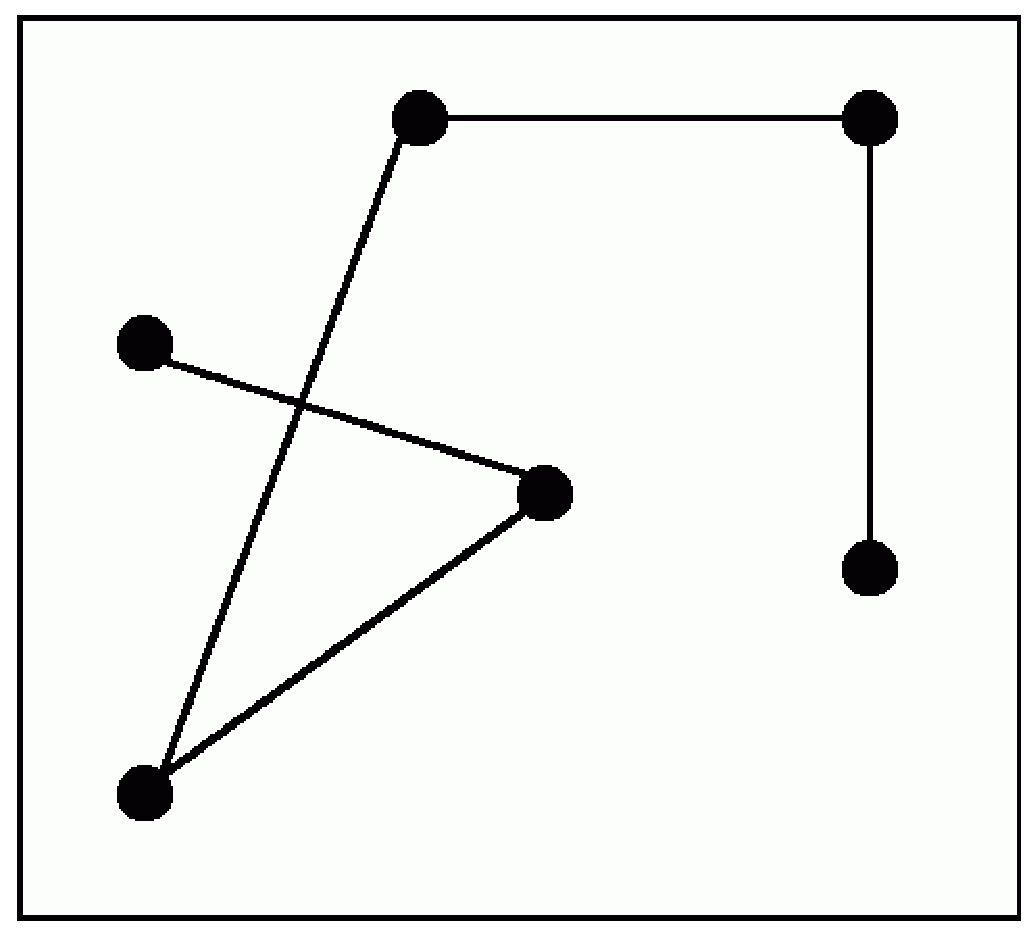
\includegraphics{pp5prob2b.gif}
\\

3.  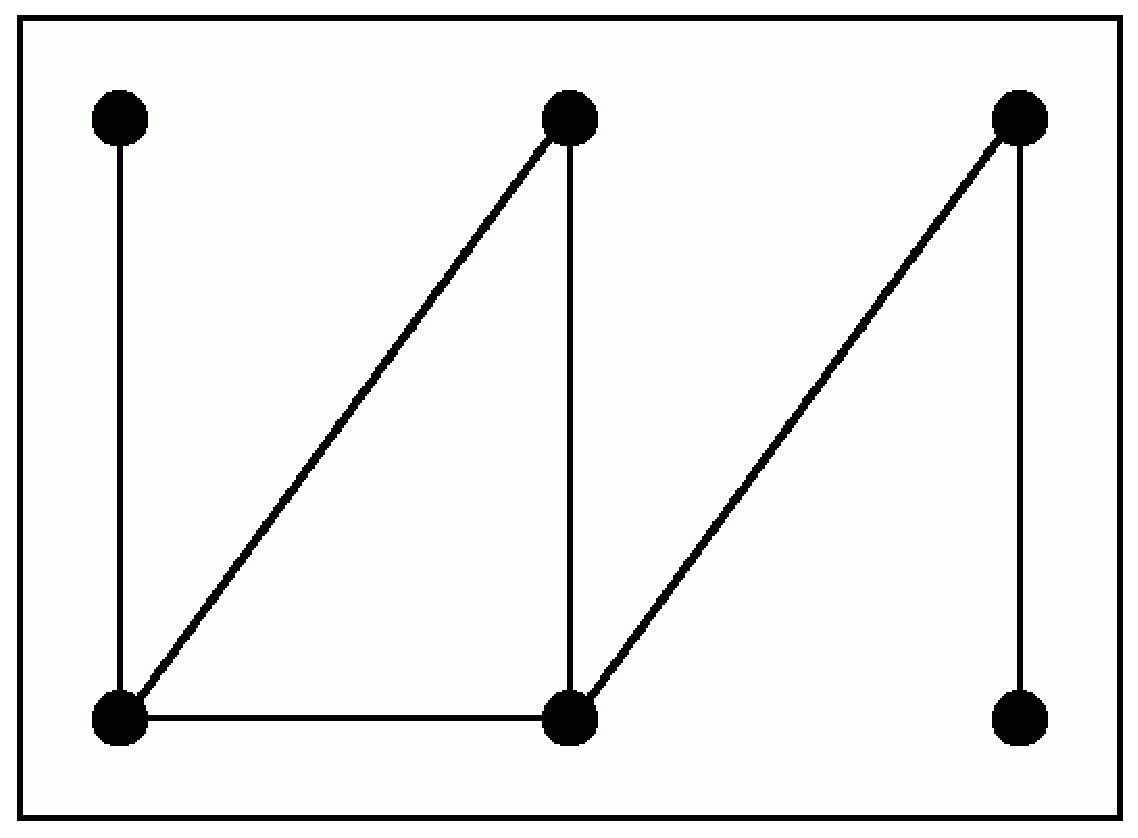
\includegraphics{pp5prob2c.gif}
& 4.  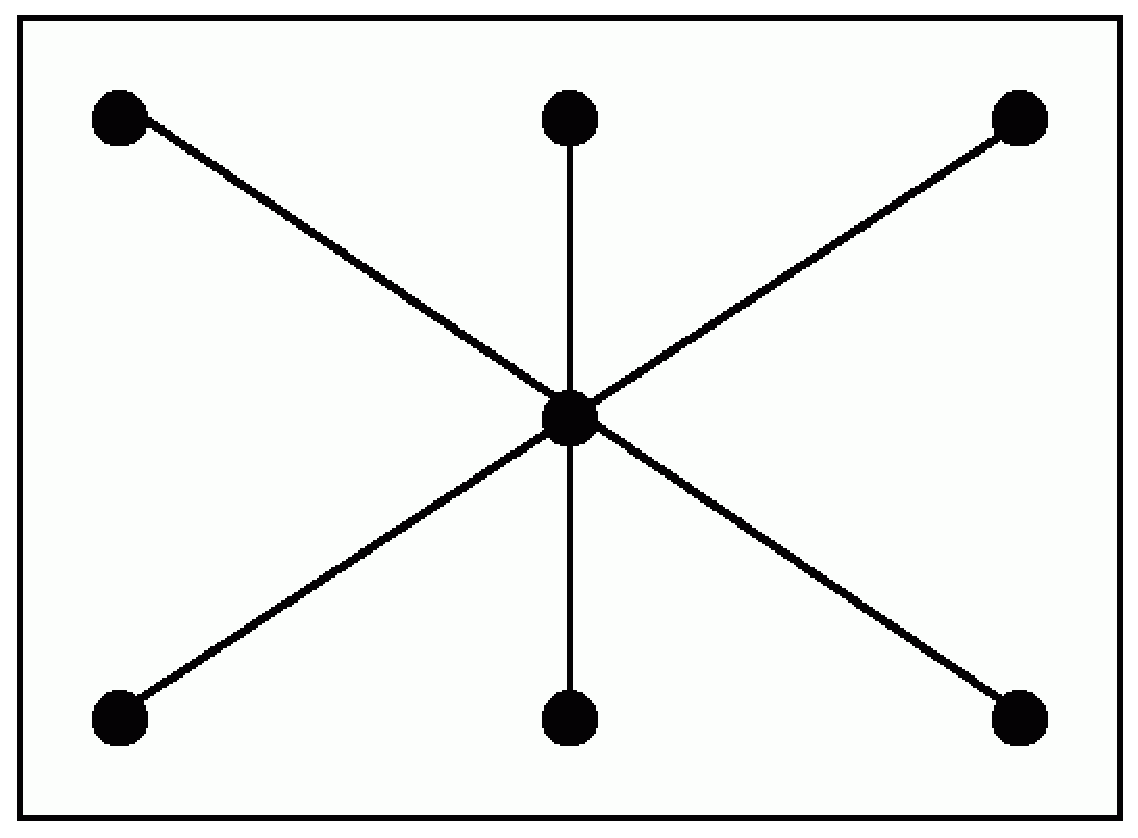
\includegraphics{pp5prob2d.gif}
\end{tabular}
\end{center}

Which of the graphs above are trees?

\begin{solution}
Graphs 2 and~4 are trees, since they are both connected and
acyclic. In contrast, graphs 1 and~3 are not trees: graph~1 is
disconnected, while graph~3 contains a cycle.
\end{solution}

%% 
%% Answer with a sequence of integers separated
%%    by some spaces, for example,
%% 
%% \begin{equation*}
%% 4 3 2 
%% 
%% \end{equation*}
%% 
%% Don't use commas or periods.
%% 

\end{problem}

\endinput
